\chapter{Apresentação dos Dados}

Para proceder à apresentação dos dados transformados utilizamos 3 plataformas, \textbf{Dashboard em C\#},
\textbf{Email} e ainda \textbf{Discord API}, neste capítulo entraremos em detalhe de como estes processos
estão definidos, assim como o seu funcionamento e apresentação.

\section*{Email}

O processo de apresentação de dados por email é feito maioritariamente através do \textbf{SPOON/KNIME}, estes transformam as tabelas de dados em texto \textbf{HTML} para poder ser apresentado da seguinte forma:

\begin{figure}[H]
    \centering
    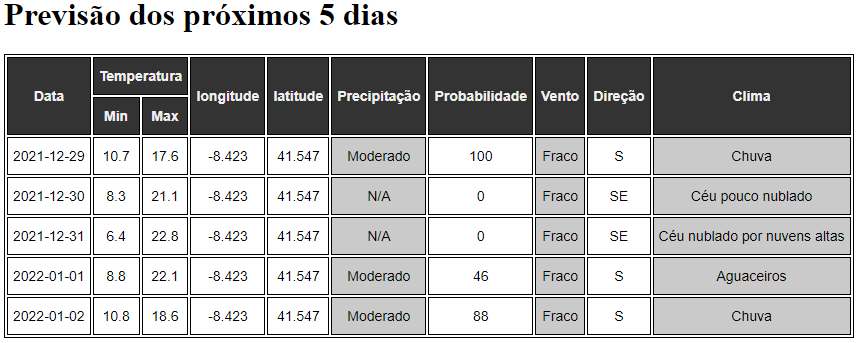
\includegraphics[scale=0.6]{imagens-spoon/email_previsao.png}
\end{figure}
\begin{figure}[H]
    \centering
    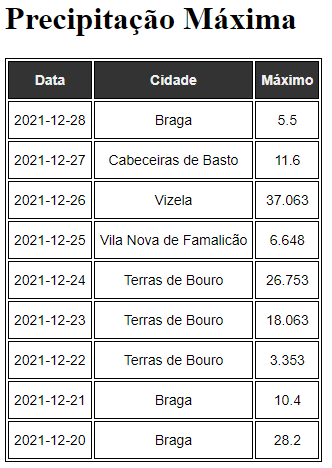
\includegraphics[scale=0.7]{imagens-spoon/email_precipitacao.png}
    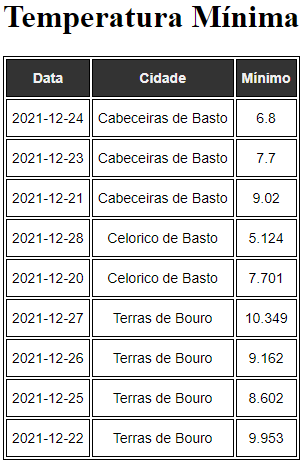
\includegraphics[scale=0.7]{imagens-spoon/email_temperatura-minima.png}
    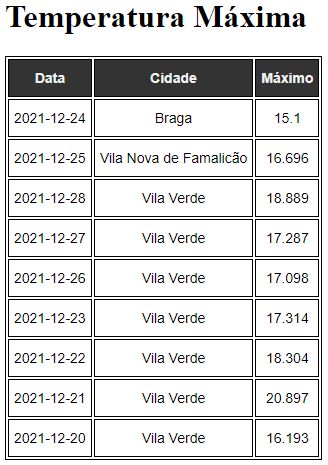
\includegraphics[scale=0.7]{imagens-spoon/emai_temp_max.png}
    \caption{Email recebido}
\end{figure}

\section*{Dashboard em C\#}
Para apresentação dos dados foi ainda utilizado um simples Dashboard feito em \textbf{Windows Forms} com 4 tabelas, uma para cada tipo de dados transformados.

O \textbf{Dashboard} tem o seguinte formato:

\begin{figure}[H]
    \centering
    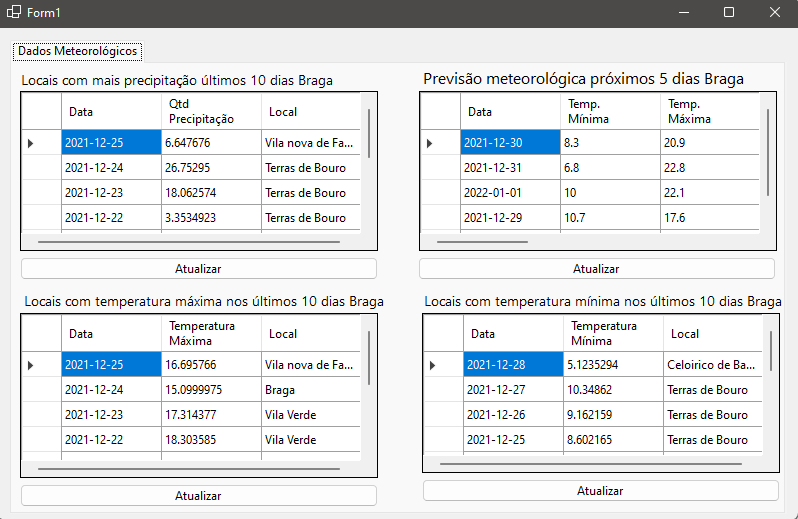
\includegraphics[scale=0.7]{imagens/Forms.png}
    \caption{Dashboard}
\end{figure}

O programa utiliza os ficheiros \textbf{JSON} guardados depois do processo de transformação de dados e converte os mesmo para as devidas \textit{Class} no C\#.

As classes utilizadas são as seguintes:

\begin{figure}[H]
    \centering
    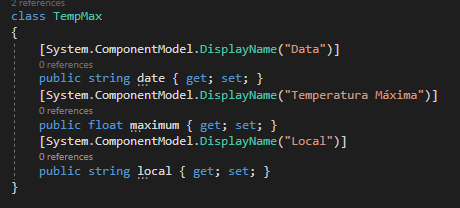
\includegraphics[scale=0.8]{imagens/TempMaxClass.png}
    \caption{\textit{Class} de Temperatura Máxima}
\end{figure}

\begin{figure}[H]
    \centering
    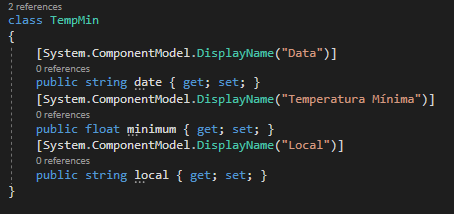
\includegraphics[scale=0.8]{imagens/TempMinClass.png}
    \caption{\textit{Class} de Temperatura Mínima}
\end{figure}

\begin{figure}[H]
    \centering
    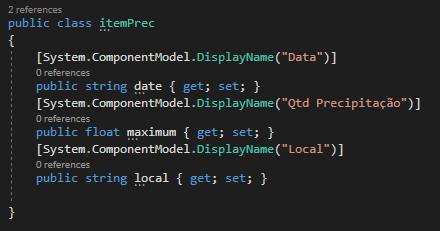
\includegraphics[scale=0.8]{imagens/PrecMaxClass.png}
    \caption{\textit{Class} de Precipitação Máxima}
\end{figure}

\begin{figure}[H]
    \centering
    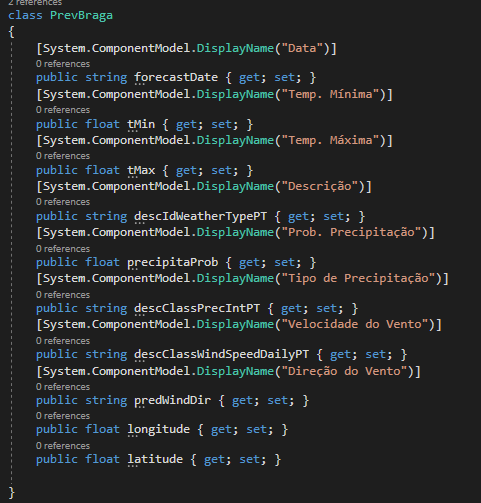
\includegraphics[scale=0.8]{imagens/PrevBragaClass.png}
    \caption{\textit{Class} de Previsão de Tempo}
\end{figure}

Depois de guardados os dados como cada uma das classes, estes são apresentados no devido \textbf{DataGridView} do \textbf{Dashboard}.

\newpage

\section*{Discord API}

\textbf{Discord} é uma plataforma de comunicação onde é possível enviar mensagens para canais de texto, assim como falar em canais de voz, esta plataforma em muito se assemelha à plataforma \textbf{Slack}. 

Assim como na plataforma Slack, o Discord disponibiliza uma API onde é possível efetuar diversas ações nos canais de comunicação. Como por exemplo a solução criada na execução deste trabalho prático, um \textbf{BOT} de envio de mensagens sobre dados meteorológicos. Para utilização da API é-nos disponibilizado um \textbf{token} de acesso com o qual fazemos a comunicação.

O \textbf{BOT} foi desenvolvido em \textbf{python} pois é disponibilizada uma biblioteca que em muito facilita a comunicação com a \textbf{Discord API}.

Assim que temos o processo do BOT a correr ele espera por um comando específico para ir buscar os dados \textbf{JSON} aos ficheiros e enviar para o utilizador, neste caso o comando é "\textbf{!tempo}". Após receber o comando o BOT envia tabelas formatadas em ASCII referentes aos dados para o canal de texto.


\begin{figure}[H]
    \centering
    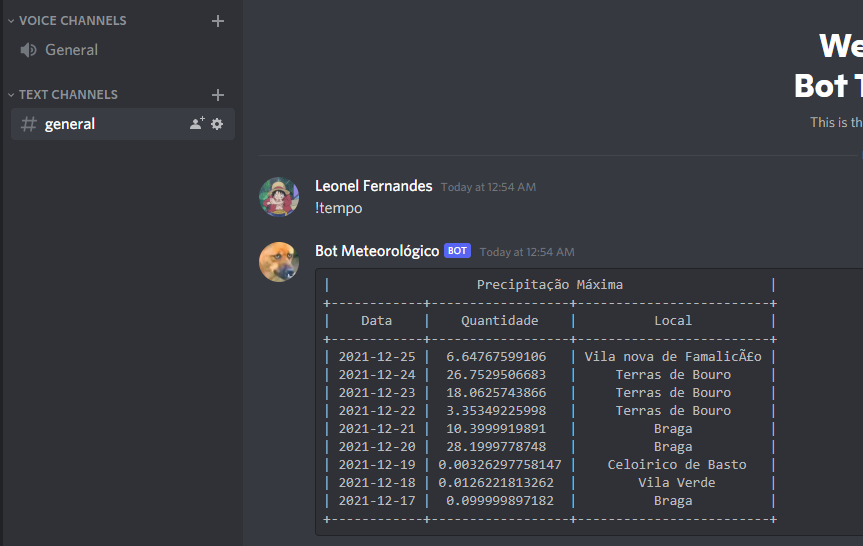
\includegraphics[scale=0.6]{imagens/Bot1.png}
    \caption{Resposta do BOT do Discord}
\end{figure}
\newpage
O BOT apresenta todas as 4 tabelas referentes aos dados. Estas tabelas são formatadas utilizando uma biblioteca do python chamada "\textbf{prettytable}".

\begin{figure}[H]
    \centering
    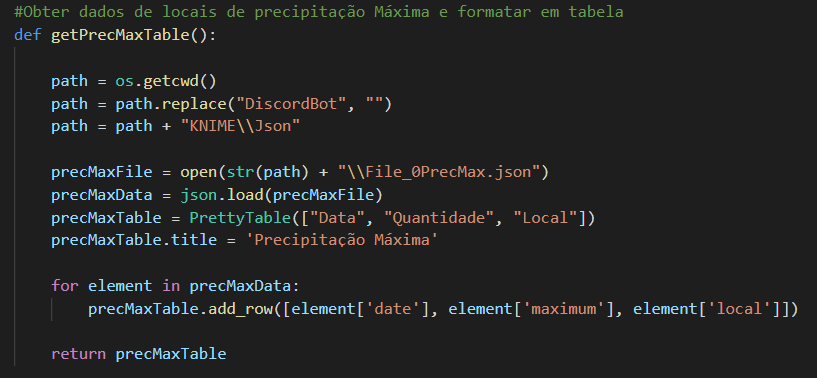
\includegraphics[scale=0.6]{imagens/formattablepython.png}
    \caption{Código de formatação de Tabela em Python}
\end{figure}

Assim como referido anteriormente, o programa tem como fonte de dados os ficheiros \textbf{JSON} para cada tabela.
\newpage

Depois de formatado apenas envia a tabela como mensagem pelo \textbf{Discord}.

\begin{figure}[H]
    \centering
    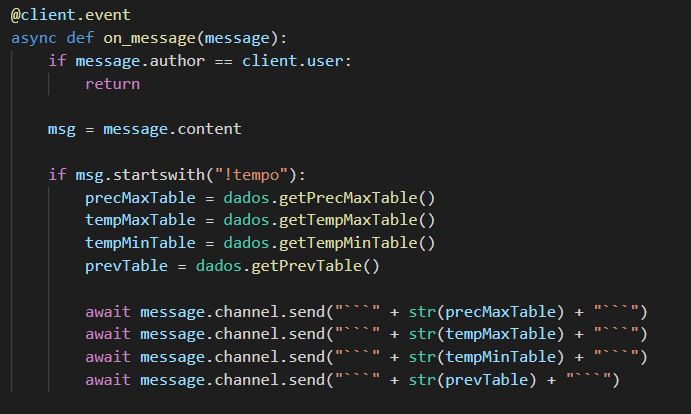
\includegraphics[scale=0.7]{imagens/tabelassenddiscord.png}
    \caption{Envio de Mensagem para o Discord}
\end{figure}
